% Roughly follows http://www.texample.net/tikz/examples/graph/
% Requirements are LaTeX (e.g. texlive), TikZ, and rubber.
% Build using the following command.
% rubber --pdf ratematrix

\documentclass{article}

\usepackage{tikz}
\usetikzlibrary{arrows,positioning}

\begin{document}
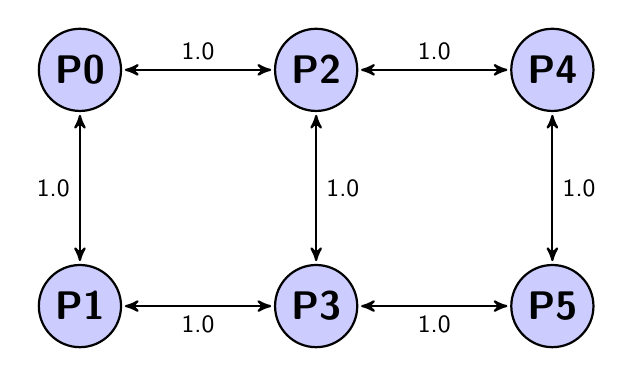
\begin{tikzpicture}[<->,>=stealth',shorten >=1pt,shorten <=1pt,
  auto,node distance=3cm,thick,
  main node/.style={circle,fill=blue!20,draw,font=\sffamily\Large\bfseries}]

  \node[main node] (0) {P0};
  \node[main node] (1) [below of=0] {P1};
  \node[main node] (2) [right of=0] {P2};
  \node[main node] (3) [below of=2] {P3};
  \node[main node] (4) [right of=2] {P4};
  \node[main node] (5) [below of=4] {P5};

  \path[every node/.style={font=\sffamily\small}]
    (0) edge node [left] {1.0} (1)
    (2) edge node [right] {1.0} (3)
    (4) edge node [right] {1.0} (5)
    (0) edge node [above] {1.0} (2)
    (2) edge node [above] {1.0} (4)
    (1) edge node [below] {1.0} (3)
    (3) edge node [below] {1.0} (5);

\end{tikzpicture}
\end{document}
